\section{Futures} \label{futures}
Consider the following arbitrary, but interesting, parallel arrow combinator:
\begin{lstlisting}[frame=htrbl]
someCombinator :: (Arrow arr) => [arr a b] -> [arr b c] -> arr [a] [c]
someCombinator fs1 fs2 = parEvalN () fs1 >>> rightRotate >>> parEvalN () fs2
\end{lstlisting}
In a distributed environment, the resulting arrow of this combinator first evaluates all \code{[arr a b]} in parallel, sends the results back to the master node, rotates the input once and then evaluates the \code{[arr b c]} in parallel to then gather the input once again on the master node. While this could be rewritten into only one \code{parEvalN} call by directly wiring the arrows properly together, this example illustrates an important problem: When using a \code{ArrowParallel} backend that resides on multiple computers, all communication between the nodes is done via the master node, as shown in figure \ref{fig:withoutFutures}. This can become a serious bottleneck in heavy threaded applications.
\begin{figure}[ht]
	\centering
	\includegraphics[width=0.9\textwidth]{images/withoutFutures}
	\caption[without Futures]{Communication between 4 threads without Futures}
	\label{fig:withoutFutures}
\end{figure}
To fix this, we have to introduce a way that enables the nodes to communicate directly with each other. Thankfully, Eden, the distributed parallel Haskell we have used in this paper so far, already ships with the concept of \code{RD} (remote data) that enables this behaviour. But as we want code written against our API to be implementation agnostic, we have to wrap this context. We do this with the \code{Future} typeclass:
\begin{lstlisting}[frame=htrbl]
class Future fut a | a -> fut where
    put :: (Arrow arr) => arr a (fut a)
    get :: (Arrow arr) => arr (fut a) a
\end{lstlisting}
As \code{RD} is only type synonym for communication type that Eden uses internally, we have to use some wrapper classes to fit that definition, though:
\begin{lstlisting}[frame=htrbl]
data RemoteData a = RD { rd :: RD a }

instance (Trans a) => Future RemoteData a where
    put = arr (\a -> RD { rd = release a })
    get = arr rd >>> arr fetch
\end{lstlisting}
For ParMonad and Multicore we can use a basic dummy wrapper as we have shared memory:
\begin{lstlisting}[frame=htrbl]
data BasicFuture a = BF { val :: a }

instance (NFData a) => Future BasicFuture a where
    put = arr (\a -> BF { val = a })
    get = arr val
\end{lstlisting}
To fit the \code{ArrowParallel} instances we gave earlier, we also have to give the necessary \code{NFData} and \code{Trans} instances - the latter only being needed in Eden.
We need this implementation for our \code{RemoteData} wrapper
\begin{lstlisting}[frame=htrbl]
instance NFData (RemoteData a) where
    rnf x = rnf $ rd x
instance Trans (RemoteData a)
\end{lstlisting}
and the following for the \code{BasicFuture} dummy type:
\begin{lstlisting}[frame=htrbl]
instance (NFData a) => NFData (BasicFuture a) where
    rnf bf = rnf $ val bf
\end{lstlisting}
Going back to our communication example we can use this new Future concept in order to enable direct communications between the nodes in the following way:
\begin{lstlisting}[frame=htrbl]
someCombinator :: (Arrow arr) => [arr a b] -> [arr b c] -> arr [a] [c]
someCombinator fs1 fs2 =
	parEvalN () (map (>>> put) fs1) >>>
	rightRotate >>>
	parEvalN () (map (get >>>) fs2)
\end{lstlisting}
In a distributed environment, this gives us a communication scheme with messages going through the master node only if it is needed - similar to what is shown in figure \ref{fig:withFutures}.
\begin{figure}[ht]
	\centering
	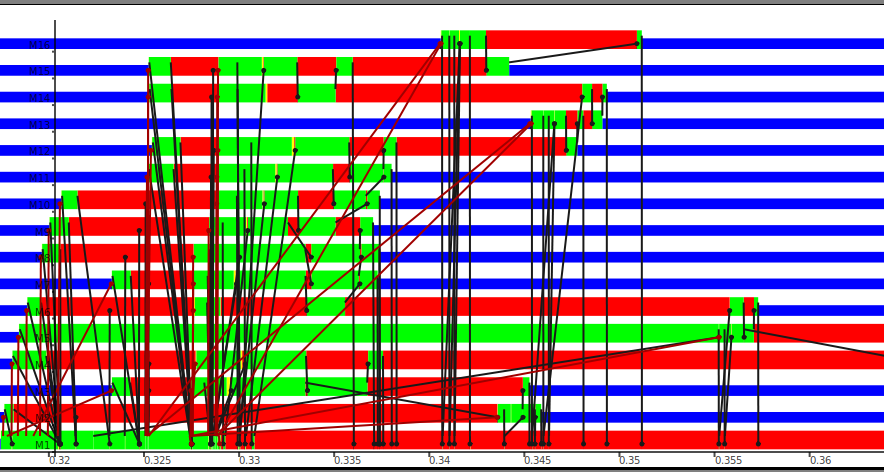
\includegraphics[width=0.9\textwidth]{images/withFutures}
	\caption[with Futures]{Communication between 4 threads with Futures}
	\label{fig:withFutures}
\end{figure}